\documentclass{beamer}
\usepackage{amsthm}
\usepackage{times}
\usepackage{graphicx}
\usefonttheme{professionalfonts}
\usetheme{metropolis}
%\usepackage{subcaption}
\usepackage{wrapfig}
\usepackage{media9}
\usepackage{tikz}
%\usecolortheme{sidebartab}
\title{Data analysis and modeling of  calcium activity in   mice somatostatin interneurons}
%\subtitle{L'equazione di Fisher}
\author[F. Bernardi]{\textbf{Fabrizio Bernardi} (944476) \\
	Advisor: Prof. Riccardo Sacco \\
	Coadvisor: Dott. Francesco Papaleo \\
	Coadvisor: Dott. Greta Chiaravalli} \medskip
%\titlegraphic{
\includegraphics[scale=.1]{Logo_Politecnico_Milano.jpg}}
%\titlegraphic{
\includegraphics[scale=.3]{Logo_IIT.png}}
%\usecolortheme{beaver}

\date[28/04/2022]{28 April, 2022}

	
\begin{document}
	
	
	\begin{frame}
	\titlepage



\end{frame}

	\begin{frame}{The GECO group}



\textbf{Genetics of Cognition (GECO)}


\begin{columns}
	\column{0.58\linewidth}
	\begin{itemize}
		\vspace{0.5cm}
		\item Held by Dr. Francesco Papaleo
		
		\vspace{0.5cm}
		
		\item Main objective: uncover the mechanisms underlying cognitive and social alterations
		
		\vspace{0.5cm}
		
		\item Empolyed methods: \textit{in vivo} studies on mice brain activity, (electrophysiology, calcium imaging ...)
		
	\end{itemize}
	\column{0.38\linewidth}
	\centering
	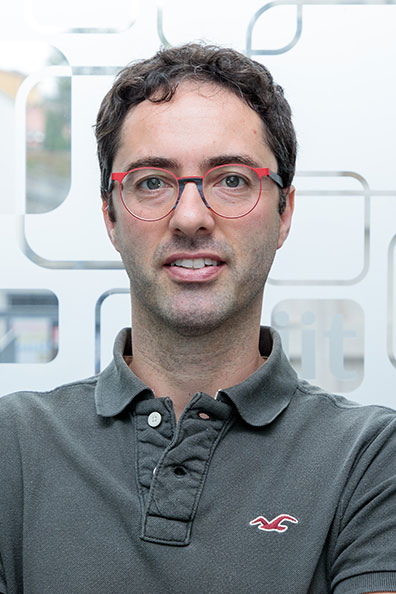
\includegraphics[scale=0.25]{papaleo}
	
\end{columns}



\end{frame}


\begin{frame}{Intracellular calcium dynamics}

\begin{columns}
	\column{0.45\linewidth}
	\begin{itemize}
		\vspace{0.5cm}
		\item Neurons show \textit{rapid} and \textit{heavy} changes in the values of their intracellular concentration of $Ca^{2+}$
		
		\vspace{0.5cm}
		
		\item The neuron is defined as \textit{active} in correspondence to the peaks in the calcium concentration
		
		
		
	\end{itemize}
	\column{0.45\linewidth}
	\centering
	\includegraphics[scale=0.4]{ca_conc}
	
\end{columns}

\end{frame}

\begin{frame}{Microendoscopic calcium imaging}



Te \textbf{Microendoscopic calcium imaging} technique consists in the following steps:

\begin{enumerate}
	
	\item Implant of \textit{miniscopes} in the brin region of interest of mice
	
	\item Injection of a virus carrying the \textbf{GCaMP} protein
	
	\item Performance of the behavioural task
	
	\item Collection of the video recordings of the occurred fluorescence activity in single neurons
	
	\item Pre-processing and data analysis
\end{enumerate}

\begin{figure}[H]
	
	\centering
	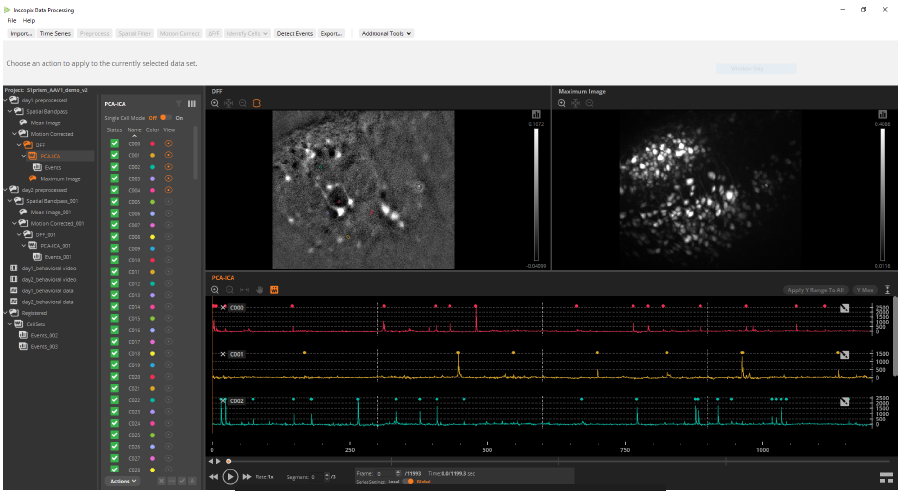
\includegraphics[width=0.25\textwidth]{inscopix}
	
\end{figure}
\end{frame}

\begin{frame}{The GECO group}

\includemedia[
width=0.6\linewidth,height=0.3375\linewidth, % 16:9
activate=pageopen,
flashvars={
	modestbranding=1 % no YT logo in control bar
	&autohide=1 % controlbar autohide
	&showinfo=0 % no title and other info before start
	&rel=0 % no related videos after end
}
]{}{http://www.youtube.com/v/r382kfkqAF4?rel=0}

\end{frame}


\end{document}



	


\begin{figure}
	
	\hfill
	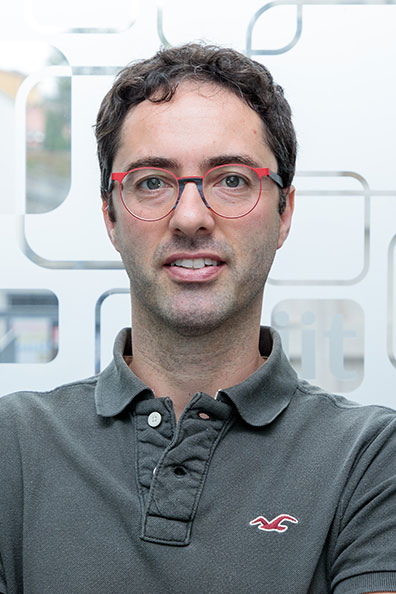
\includegraphics[width=0.25\textwidth]{papaleo.jpg}
	
\end{figure}


\begin{frame}{The GECO group}
	contenuto...
\end{frame}